% !TeX spellcheck = de_CH_frami

\section{Laplace Operator und Graphen\label{sec:sgwt:laplace}}
\rhead{Laplace Operator und Graphen}

F\"ur die Analyse und Synthese von Funktionen auf Graphen und deren Spektren 
spielen der 
Laplace Operator und besonders die Laplace Matrix eine wichtige Rolle, wie 
bereits Graphen in~\cref{sec:sgwt:graphs}, wollen wir daher zuerst 
die Grundlagen des Laplace Operators in~\cref{subsec:sgwt:laplaceop} und der 
Laplace Matrix \laplaceL{} in~\cref{subsec:sgwt:laplacem} eingehen, bevor wir 
dann in~\cref{sec:sgwt:spectralanalysis} mit der Analyse des Spektrums und 
Konstruktion der SGWT beginnen.

\subsection{Laplace Operator\label{subsec:sgwt:laplaceop}}
\rhead{Laplace Operator}

Der Laplace Operator $\Delta$ in $\mathbb{R}^n$ wird im kartesischen 
Koordinatensystem durch die Summe der $n$~zweiten Ableitungen
\begin{equation*}
\Delta = 
\sum_{i = 1}^{n}\frac{\partial^2}{\partial x_i^2}
=
\frac{\partial^2}{\partial x_1^2}
+ \frac{\partial^2}{\partial x_2^2}
+ \dots
+ \frac{\partial^2}{\partial x_n^2}
\end{equation*}
beschrieben. H\"aufig trifft man erstmals auf den Laplace Operator wenn man 
versucht die Poisson-Gleichung $-\Delta u = f$ zu l\"osen.

Wie Anfangs bereits beschrieben, sind unsere Daten meist nur in diskreter Form 
vorhanden. Daher w\"are es vorteilhaft, auch eine diskretisierte oder zumindest 
approximierte Form des Laplace Operators zu haben.

\subsection{Finite-Differenzen}
\rhead{Finite-Differenzen}

Finite-Differenzen erm\"oglichen uns eine diskrete Approximation des 
Laplace Operators. Sie stellen also eine L\"osung f\"ur unsere Problem dar, auf 
die wir weiter eingehen wollen.

Als Ausgangslage nehmen wir die Funktion $u(x)$ mit dem eindimensionalen 
Definitionsbereich $u: \mathbb{R} \rightarrow \mathbb{R}$ und beginnen zuerst 
mit der Approximation der ersten Ableitung an der Stelle $x_i$, mit dem Abstand 
$h = \Delta x_i$,
\begin{equation*}
\frac{\partial u}{\partial x_i}
= \frac{u(x_i+h)-u(x_i)}{h}.
\end{equation*}
Indem wir diese Gleichung nochmals ableiten, erhalten wir die f\"ur den Laplace 
Operator relevante zweite Ableitung
\begin{equation*}
\frac{\partial}{\partial x_i}\frac{\partial}{\partial x_i}u
= \frac{\partial^2 u}{\partial x_i^2}
= \frac{\frac{u(x_i+h)-u(x_i)}{h}-\frac{u(x_i)-u(x_i+h)}{h}}{h}
= \frac{u(x_i+h)-2u(x_i)+u(x_i-h)}{h^2}.
\end{equation*}

Dies k\"onnen wir nat\"urlich auch in zwei Dimensionen mit Funktionen der Art 
$u(x, y)$ machen. Wieder wenden wir zuerst den Laplace Operator $\Delta$ auf 
unser $u$ an und erhalten
\begin{equation*}
\Delta u(x, y) = u_{xx}(x, y) + u_{yy}(x, y).
\end{equation*}
Dies k\"onnen wir wiederum mittels Finiten-Differenzen approximieren, mit $h = 
\Delta x = \Delta y$ liefert uns das
\begin{align}
\Delta u(x,y)
&=
\frac{u(x+h,y)-2u(x, y)+u(x-h,y)}{h^2}
+\frac{u(x,y+h)-2u(x, y)+u(x,y-h)}{h^2} \nonumber \\
&=
\frac{u(x+h,y)+u(x-h,y)+u(x,y+h)+u(x,y-h)-4u(x, y)}{h^2}.
\label{eq:sgwt:fivepointstencil}
\end{align}
Dieser Operator ist auch bekannt als der F\"unfpunkte-Stern-Operator 
oder five-point stencil im Englischen, siehe~\cref{fig:sgwt:graph:star}.
\begin{figure}
\centering
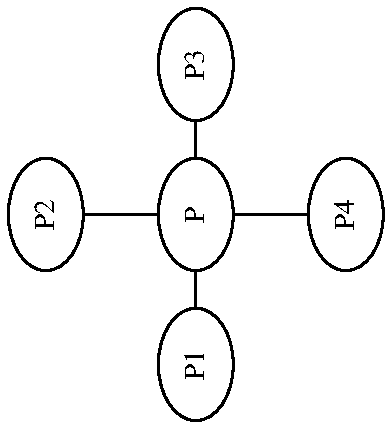
\includegraphics[
angle=-90,
origin=c,
scale=0.6
]{papers/sgwt/images/star.pdf}
\vspace{0pt}
\caption{F\"unfpunkte-Stern-Operator mit $P = u(x,y), P_1 = 
u(x-h,y), P_2 = u(x,y+h), P_3 = u(x+h,y), P_4 = u(x,y-h)$.
\label{fig:sgwt:graph:star}}
\end{figure}

Es folgt daraus, dass bei der zweiten Ableitung die ``aufeinanderfolgenden 
Differenzen'' immer den Knoten in der Mitte gemeinsam haben. Damit k\"onnen 
wir nun wieder zur\"uck auf unsere Graphen 
in~\cref{fig:sgwt:graph:simple} aus~\cref{sec:sgwt:graphs} kommen. Wenn wir 
diesen n\"amlich mit dem den F\"unfpunkte-Stern-Operator 
aus~\cref{fig:sgwt:graph:star} vergleichen, wird klar, dass der Graph, obwohl 
er auf den ersten Blick anders aussieht, der Gleiche ist. Wenn wir also den 
Laplace Operator auf den jeweiligen Graph anwenden, werden wir das gleiche 
Resultat erhalten.

Wir k\"onnen somit noch einen Schritt weitergehen und uns von den Achsen 
l\"osen. Nehmen wir als Beispiel den Graphen aus~\cref{fig:sgwt:laplace:nstar}. 
F\"ur die zweite Ableitung beim Punkt P brauchen wir also nach dem Schema 
aus~\cref{eq:sgwt:fivepointstencil} die Summe aller Funktionswerte $u(P_1)$ bis 
$u(P_8)$ abz\"uglich Anzahl Nachbarn von $P$, also dem Grad $d(P)$, 
multipliziert mit dem Funktionswert $u(P)$, was uns folgende Gleichung
\begin{equation*}
\Delta u = \frac{1}{h^2}\left(\sum_{i = 1}^{8}u(P_i) - 8u(P)\right)
\end{equation*}
liefert. Generell erhalten wir f\"ur den Laplace Operator an einem Knoten $v$ 
mit $n$~Nachbarn die folgende~\cref{eq:sgwt:generallaplace}.
\begin{equation}
\Delta u = \frac{1}{h^2}\left(\sum_{i = 1}^{n}u(v_i) - d(v)u(v)\right)
\label{eq:sgwt:generallaplace}
\end{equation}

\begin{figure}
\centering
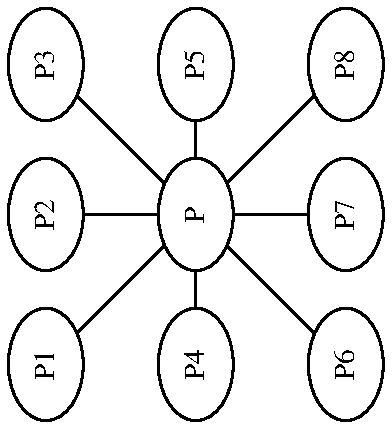
\includegraphics[
angle=-90,
origin=c,
scale=0.7
]{papers/sgwt/images/nstar.pdf}
\vspace{0pt}
\caption{Ein Graph mit neun Knoten und acht Kanten. Der Knote P mit Grad 
$d(P) = 8$ sticht hier klar gegen\"uber den anderen Knoten mit jeweils 
Grad $d(\text{P}_i) = 1$ hervor.
    \label{fig:sgwt:laplace:nstar}}
\end{figure}

\subsection{Laplace Matrix\label{subsec:sgwt:laplacem}}
\rhead{Laplace Matrix}

Wenn wir nun mit Hilfe von Taschenrechnern oder Computer rechnen wollen, ist 
meist die Darstellung in Form einer Matrix besonders geeignet.
Die Laplace Matrix \laplaceL{}~\cite{noauthor_laplace-matrix_2017} ist genau 
dies, sie beschreibt einen Graphen anhand seiner Gradmatrix 
\degreeM{}~\cite{noauthor_degree_2018} und Adjazenzmatrix 
\adjacencyM{}~\cite{noauthor_adjacency_2019} wie folgt
\begin{equation}
\laplaceL = \degreeM - \adjacencyM.
\label{eq:sgwt:laplace}
\end{equation}

Die Gradmatrix \degreeM{} ist dabei eine Diagonalmatrix, die den Grad der 
einzelnen Knoten beinhaltet. Die Adjazenzmatrix hingegen zeigt die Kanten und 
deren Gewichte des Graphen auf. Als Beispiel dient uns 
wieder der Graph aus~\cref{fig:sgwt:graph:simple}, dessen Grad- und 
Adjazenzmatrix wie folgt
\begin{equation*}
\degreeM =
\begin{bmatrix}
1 & 0 & 0 & 0 & 0 \\
0 & 4 & 0 & 0 & 0 \\
0 & 0 & 1 & 0 & 0 \\
0 & 0 & 0 & 1 & 0 \\
0 & 0 & 0 & 0 & 1
\end{bmatrix}
\end{equation*}
sowie
\begin{equation*}
\adjacencyM =
\begin{bmatrix}
0 & 1 & 0 & 0 & 0 \\
1 & 0 & 1 & 1 & 1 \\
0 & 1 & 0 & 0 & 0 \\
0 & 1 & 0 & 0 & 0 \\
0 & 1 & 0 & 0 & 0
\end{bmatrix}
\end{equation*}
aussehen. Die Differenz der beiden ergibt dann die Laplace Matrix
\begin{equation*}
\laplaceL =
\begin{bmatrix}
1 & -1 & 0 & 0 & 0 \\
-1 & 4 & -1 & -1 & -1 \\
0 & -1 & 1 & 0 & 0 \\
0 & -1 & 0 & 1 & 0 \\
0 & -1 & 0 & 0 & 1
\end{bmatrix}.
\end{equation*}
Wenden wir nun die Funktion $u$ auf diese Matrix an, erhalten wir
\begin{equation*}
\laplaceL u =
\begin{bmatrix}
1 & -1 & 0 & 0 & 0 \\
-1 & 4 & -1 & -1 & -1 \\
0 & -1 & 1 & 0 & 0 \\
0 & -1 & 0 & 1 & 0 \\
0 & -1 & 0 & 0 & 1
\end{bmatrix}
\begin{pmatrix}
u_0 \\
u_1 \\
u_2 \\
u_3 \\
u_4
\end{pmatrix}
=
\begin{pmatrix}
u_0 - u_1 \\
4 u_1 - u_0 - u_2 - u_3 - u_4 \\
u_2 - u_1 \\
u_3 - u_1 \\
u_4 - u_1
\end{pmatrix}
\end{equation*}
oder generell ausgedr\"uckt, mit $h = 1$
\begin{equation*}
\laplaceL u = \frac{1}{h^2}n\left(\frac{1}{n}\sum_{i\text{ Nachbarn}}^{n}u_i - 
u_0\right) = \Delta u.
\end{equation*}
